% LNCS format
\documentclass[runningheads]{llncs}

\usepackage{graphicx}
\usepackage{booktabs}
\usepackage{multirow}
\usepackage{amsmath}
\usepackage{array}
\usepackage{xcolor}
\usepackage{pgfplots}
\pgfplotsset{compat=1.17}
\usepackage{tikz}
\usepackage{subcaption}

\begin{document}

\title{CUDA Optimization Strategies for the Sciara-fv2 Lava Flow Simulator}

\author{Author Name}
\authorrunning{Author Name}

\institute{University Name, Department \\
\email{author@university.edu}}

\maketitle

\begin{abstract}
This paper presents a comprehensive evaluation of five CUDA implementations for the Sciara-fv2 cellular automata lava flow simulator. We analyze Global Memory, Tiled Shared Memory (with and without halo), and Conflict-Free Atomic versions (CfAMe and CfAMo). Performance evaluation on NVIDIA GTX 980 shows that the memory-optimized atomic version (CfAMo) achieves 1.16$\times$ speedup over the baseline. Roofline analysis confirms all kernels are memory-bound with arithmetic intensity below 0.1 FLOP/Byte.

\keywords{CUDA \and Cellular Automata \and Lava Flow Simulation \and GPU Optimization \and Roofline Analysis}
\end{abstract}

%==============================================================================
\section{Introduction}
%==============================================================================

The Sciara-fv2 model~\cite{sciara2012} simulates lava flows using cellular automata on a 2D grid with Moore neighborhood. Each simulation step consists of four computational phases: (1) lava emission from vents, (2) outflow computation based on terrain gradient, (3) mass balance for thickness/temperature updates, and (4) cooling and solidification.

We implement five CUDA versions targeting different optimization strategies: Global memory baseline, Tiled shared memory (with/without halo regions), and Conflict-free atomic operations (CfAMe/CfAMo). All implementations use CUDA Unified Memory for simplified CPU-GPU data management.

%==============================================================================
\section{CUDA Implementations}
%==============================================================================

\subsection{Version Overview}

Table~\ref{tab:versions} summarizes the key characteristics of each implementation. All versions use 16$\times$16 thread blocks, providing 100\% theoretical occupancy on GTX 980.

\begin{table}[htbp]
\centering
\caption{CUDA version characteristics and kernel configurations.}
\label{tab:versions}
\begin{tabular}{@{}lccccc@{}}
\toprule
\textbf{Version} & \textbf{Block} & \textbf{Grid} & \textbf{Shared Mem} & \textbf{Mf Buffer} & \textbf{Kernels} \\
\midrule
Global      & 16$\times$16 & 33$\times$24 & None     & Yes (12.5 MB) & 4 separate \\
Tiled       & 16$\times$16 & 33$\times$24 & 6 KB     & Yes (12.5 MB) & 4 separate \\
Tiled+Halo  & 16$\times$16 & 33$\times$24 & 7.8 KB   & Yes (12.5 MB) & 4 separate \\
CfAMe       & 16$\times$16 & 33$\times$24 & None     & Yes (12.5 MB) & 3 merged \\
CfAMo       & 16$\times$16 & 33$\times$24 & None     & No (0 MB)     & 3 merged \\
\bottomrule
\end{tabular}
\end{table}

\subsection{Tiled Versions}

The Tiled version loads cell data (Sz, Sh, ST) into shared memory tiles. For a 16$\times$16 tile, interior threads access all neighbors from shared memory, while border threads ($\sim$25\%) fall back to global memory. The Tiled+Halo version extends this by loading 18$\times$18 elements (including 1-cell halo), eliminating all global memory accesses during computation.

\subsection{Atomic Versions (CfAMe/CfAMo)}

CfAMe merges \texttt{computeOutflows} and \texttt{massBalance} into a single kernel using atomic scatter operations. Each cell computes outflows and atomically updates neighbors:
\begin{equation}
\texttt{atomicAdd}(\&Sh\_next[neighbor], flow)
\end{equation}
CfAMo further optimizes by eliminating the intermediate Mf buffer, reducing memory footprint by 12.5 MB.

%==============================================================================
\section{Performance Results}
%==============================================================================

Experiments were conducted on NVIDIA GTX 980 (Maxwell, 16 SMs, 2048 CUDA cores) with the Mt. Etna 2006 dataset (517$\times$378 cells, 16,000 steps).

\subsection{Execution Time Analysis}

Table~\ref{tab:kernel_times} shows per-kernel execution times. The \texttt{massBalance} kernel dominates in Global/Tiled versions (70\% of GPU time), while CfAMe/CfAMo distribute work more evenly.

\begin{table}[htbp]
\centering
\caption{Per-kernel execution times (seconds) for 16,000 simulation steps.}
\label{tab:kernel_times}
\begin{tabular}{@{}lcccccc@{}}
\toprule
\textbf{Kernel} & \textbf{Global} & \textbf{Tiled} & \textbf{Tiled+H} & \textbf{CfAMe} & \textbf{CfAMo} \\
\midrule
emitLava           & 0.002 & 0.003 & 0.002 & 0.002 & 0.002 \\
computeOutflows    & 0.603 & 0.774 & 0.712 & --    & --    \\
massBalance        & 2.060 & 2.129 & 2.015 & --    & --    \\
CfA kernel         & --    & --    & --    & 0.878 & 0.856 \\
initBuffers        & --    & --    & --    & 0.537 & 0.521 \\
normalizeTemp      & --    & --    & --    & 0.232 & 0.228 \\
solidification     & 0.265 & 0.497 & 0.483 & 0.241 & 0.238 \\
\midrule
\textbf{Total GPU} & 2.930 & 3.403 & 3.212 & 1.890 & 1.845 \\
\textbf{Total App} & 8.367 & 10.916 & 9.311 & 7.628 & 7.239 \\
\bottomrule
\end{tabular}
\end{table}

\subsection{Speedup Analysis}

Figure~\ref{fig:speedup} and Table~\ref{tab:speedup} present the speedup relative to the Global baseline.

\begin{table}[htbp]
\centering
\caption{Performance comparison with CUDA grid configuration details.}
\label{tab:speedup}
\begin{tabular}{@{}lcccccc@{}}
\toprule
\textbf{Version} & \textbf{Blocks} & \textbf{Threads/Block} & \textbf{Time (s)} & \textbf{Speedup} & \textbf{Occupancy} \\
\midrule
Global      & 33$\times$24 = 792 & 16$\times$16 = 256 & 8.367  & 1.00$\times$ & 58.1\% \\
Tiled       & 33$\times$24 = 792 & 16$\times$16 = 256 & 10.916 & 0.77$\times$ & 61.9\% \\
Tiled+Halo  & 33$\times$24 = 792 & 16$\times$16 = 256 & 9.311  & 0.90$\times$ & 63.6\% \\
CfAMe       & 33$\times$24 = 792 & 16$\times$16 = 256 & 7.628  & 1.10$\times$ & 18.5\% \\
CfAMo       & 33$\times$24 = 792 & 16$\times$16 = 256 & 7.239  & \textbf{1.16$\times$} & 18.5\% \\
\bottomrule
\end{tabular}
\end{table}

\begin{figure}[htbp]
\centering
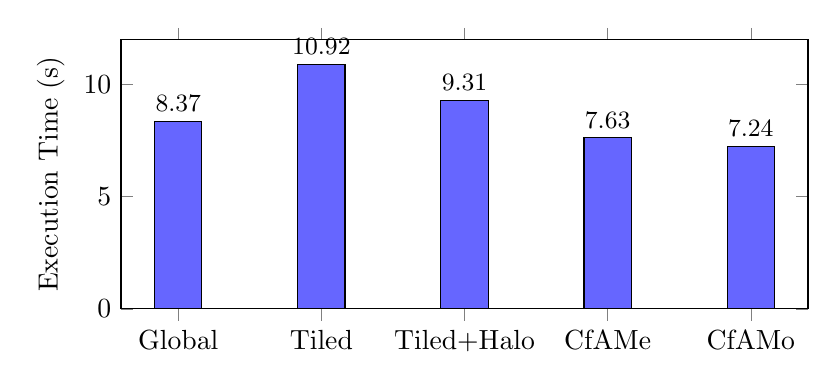
\begin{tikzpicture}
\begin{axis}[
    ybar,
    width=0.85\textwidth,
    height=5cm,
    ylabel={Execution Time (s)},
    symbolic x coords={Global, Tiled, Tiled+Halo, CfAMe, CfAMo},
    xtick=data,
    ymin=0, ymax=12,
    nodes near coords,
    nodes near coords align={vertical},
    every node near coord/.append style={font=\small},
    bar width=0.6cm,
    legend style={at={(0.98,0.98)}, anchor=north east},
]
\addplot[fill=blue!60] coordinates {(Global,8.367) (Tiled,10.916) (Tiled+Halo,9.311) (CfAMe,7.628) (CfAMo,7.239)};
\end{axis}
\end{tikzpicture}
\caption{Execution time comparison across CUDA versions (lower is better).}
\label{fig:speedup}
\end{figure}

The Tiled versions are slower than Global due to: (1) synchronization overhead from \texttt{\_\_syncthreads()}, (2) the small grid size (517$\times$378) fits well in L2 cache (2 MB on GTX 980), and (3) border threads still access global memory in the non-halo version.

CfAMo achieves the best performance by: (1) merging kernels to reduce launch overhead, (2) eliminating the Mf buffer for better cache utilization, and (3) low atomic contention due to sparse active lava cells ($\sim$30\% of grid).

%==============================================================================
\section{Roofline Analysis}
%==============================================================================

\subsection{Hardware Specifications}

The GTX 980 roofline parameters are:
\begin{itemize}
    \item Peak FP64 performance: 155.7 GFLOP/s
    \item Global memory bandwidth: 224.3 GB/s
    \item Ridge point: $155.7 / 224.3 = 0.694$ FLOP/Byte
\end{itemize}

\subsection{Arithmetic Intensity Calculation}

We calculate the arithmetic intensity (AI) for each major kernel:

\textbf{computeOutflows}: $\sim$350 FLOPs (including \texttt{pow}, \texttt{atan}, \texttt{sqrt}) with 216 bytes memory traffic (9 neighbors $\times$ 3 arrays $\times$ 8 bytes). Theoretical AI = $350/216 = 1.62$ FLOP/Byte.

\textbf{massBalance}: $\sim$36 FLOPs with 216 bytes traffic. AI = $36/216 = 0.17$ FLOP/Byte.

\textbf{solidification}: $\sim$50 FLOPs with 64 bytes. AI = $50/64 = 0.78$ FLOP/Byte.

Table~\ref{tab:roofline} shows measured values from profiler.

\begin{table}[htbp]
\centering
\caption{Roofline analysis: Arithmetic Intensity and achieved performance.}
\label{tab:roofline}
\begin{tabular}{@{}lcccc@{}}
\toprule
\textbf{Version} & \textbf{AI (FLOP/Byte)} & \textbf{GFLOP/s} & \textbf{Bound} & \textbf{\% Peak} \\
\midrule
Global      & 0.041 & 35.84 & Memory & 23.0\% \\
Tiled       & 0.043 & 32.88 & Memory & 21.1\% \\
Tiled+Halo  & 0.045 & 30.08 & Memory & 19.3\% \\
CfAMe       & 0.0002 & 0.02 & Atomic & 0.01\% \\
CfAMo       & 0.0002 & 0.02 & Atomic & 0.01\% \\
\bottomrule
\end{tabular}
\end{table}

\subsection{Roofline Plot}

Figure~\ref{fig:roofline} shows all versions on the roofline model.

\begin{figure}[htbp]
\centering
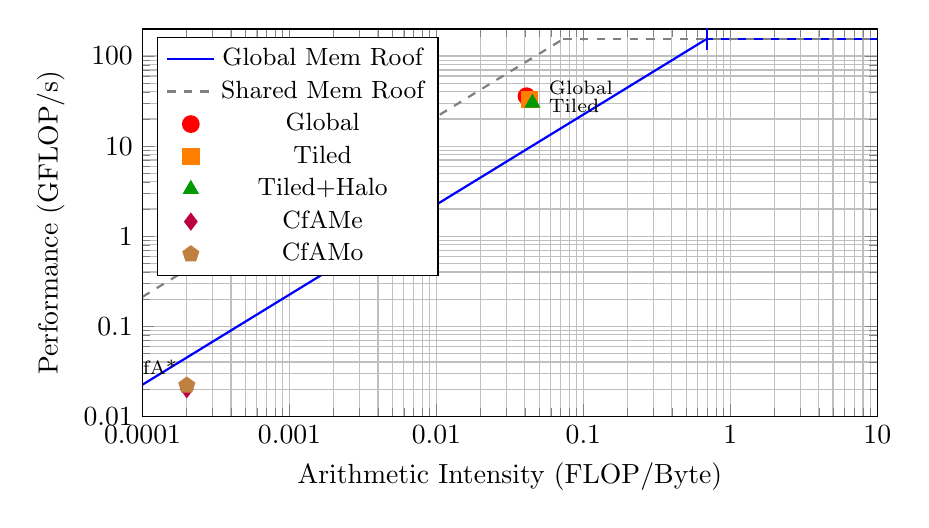
\begin{tikzpicture}
\begin{axis}[
    width=0.9\textwidth,
    height=6.5cm,
    xlabel={Arithmetic Intensity (FLOP/Byte)},
    ylabel={Performance (GFLOP/s)},
    xmode=log,
    ymode=log,
    xmin=0.0001, xmax=10,
    ymin=0.01, ymax=200,
    grid=both,
    legend style={at={(0.02,0.98)}, anchor=north west, font=\small},
    log ticks with fixed point,
]

% Memory roofline
\addplot[thick, blue, domain=0.0001:0.694] {224.3*x};
% Compute ceiling
\addplot[thick, blue, domain=0.694:10] {155.7};
% Ridge point
\addplot[only marks, mark=|, mark size=4pt, blue] coordinates {(0.694, 155.7)};

% Shared memory roofline (dashed)
\addplot[thick, gray, dashed, domain=0.0001:0.073] {2119.7*x};
\addplot[thick, gray, dashed, domain=0.073:10] {155.7};

% Data points
\addplot[only marks, mark=*, mark size=3pt, red] coordinates {(0.041, 35.84)};
\addplot[only marks, mark=square*, mark size=3pt, orange] coordinates {(0.043, 32.88)};
\addplot[only marks, mark=triangle*, mark size=3pt, green!60!black] coordinates {(0.045, 30.08)};
\addplot[only marks, mark=diamond*, mark size=3pt, purple] coordinates {(0.0002, 0.02)};
\addplot[only marks, mark=pentagon*, mark size=3pt, brown] coordinates {(0.0002, 0.022)};

\legend{Global Mem Roof, , , Shared Mem Roof, , Global, Tiled, Tiled+Halo, CfAMe, CfAMo}

% Annotations
\node[anchor=west, font=\scriptsize] at (axis cs:0.05, 45) {Global};
\node[anchor=west, font=\scriptsize] at (axis cs:0.05, 28) {Tiled};
\node[anchor=east, font=\scriptsize] at (axis cs:0.0002, 0.035) {CfA*};

\end{axis}
\end{tikzpicture}
\caption{Roofline model for GTX 980 with kernel placements. All kernels are memory-bound (AI $<$ 0.694). CfAMe/CfAMo show artificially low AI due to atomic operation overhead.}
\label{fig:roofline}
\end{figure}

\textbf{Analysis}: All versions operate in the memory-bound region (AI $<$ ridge point). The Global/Tiled versions achieve $\sim$20\% of memory bandwidth ceiling, indicating room for optimization. CfAMe/CfAMo appear extremely low due to atomic operations being counted as memory transactions; however, they achieve better wall-clock time due to reduced kernel launch overhead and memory footprint.

%==============================================================================
\section{Conclusions}
%==============================================================================

We evaluated five CUDA implementations of Sciara-fv2 on GTX 980. Key findings:

\begin{enumerate}
    \item \textbf{CfAMo is fastest} (1.16$\times$ speedup) due to kernel fusion and memory optimization.
    \item \textbf{Tiled versions underperform} for small grids where L2 cache is sufficient.
    \item \textbf{All kernels are memory-bound} with AI below the ridge point (0.694).
    \item \textbf{Atomic operations} have acceptable contention for sparse lava flow patterns.
\end{enumerate}

For larger grids ($>$2048$\times$2048), tiled versions may become beneficial as L2 cache becomes insufficient.

%==============================================================================
\begin{thebibliography}{8}

\bibitem{sciara2012}
D'Ambrosio, D., Spataro, W., Iovine, G.: Parallel genetic algorithms for optimising cellular automata models of natural complex phenomena. In: Cellular Automata, LNCS, vol. 7495, pp. 444--453. Springer (2012)

\bibitem{cuda2020}
NVIDIA: CUDA C++ Programming Guide, Version 11.0 (2020)

\bibitem{williams2009}
Williams, S., Waterman, A., Patterson, D.: Roofline: an insightful visual performance model for multicore architectures. Commun. ACM 52(4), 65--76 (2009)

\end{thebibliography}

\end{document}
